% !TeX program = pdflatex
% Build from this folder with pdflatex CA1-Report.tex (run twice for references).
% Replace the bracketed prompts and author details before submission.
\documentclass[11pt,a4paper]{article}

\usepackage[T1]{fontenc}
\usepackage{lmodern}
\usepackage[margin=24mm]{geometry}
\usepackage{graphicx}
\usepackage{booktabs}
\usepackage{tabularx}
\usepackage{pdflscape}
\usepackage[hidelinks]{hyperref}

\title{\textbf{Distributed Transaction Coordination}\\[3pt]
  \large Modeling and Formal Verification\\
  \normalsize Programming Assignment 1, Part 1}
\author{[First student name] \\ {[Student number]}
  \and [Second student name] \\ {[Student number]}}
\date{University of Tehran \enspace\textbullet\enspace Fall 1405}

% Viewports show the MSCs and crop the surrounding SpinRCP interface.
\newcommand{\scenariochart}[4]{%
  \begin{minipage}[t]{0.48\textwidth}
    \vspace{0pt}%
    \centering
    \includegraphics[viewport={#2},clip,width=\linewidth,
      height=0.60\textheight,keepaspectratio]{#1}%
    \caption{#3}\label{#4}
  \end{minipage}%
}

\newcommand{\servicegraph}[3]{%
  \begin{figure}[!ht]
    \centering
    \includegraphics[page=#1,width=0.93\linewidth]{CA1-Program-Graphs.pdf}
    \caption{#2}\label{#3}
  \end{figure}%
}

\begin{document}
\maketitle

\section{Model Design}
\label{sec:model}

\subsection{Promela Processes}
[Explain the roles of the Transaction Coordinator and the Inventory,
Payment, and Shipping services. Refer to the program graphs in
Appendix~\ref{app:graphs} when describing their control flow.]

\subsection{Channels and Message Types}
[Explain the rendezvous channels \texttt{inv}, \texttt{pay}, and
\texttt{ship}. Describe who sends and receives \texttt{EXECUTE},
\texttt{SUCCESS}, \texttt{FAILURE}, \texttt{COMPENSATE},
\texttt{COMPENSATED}, \texttt{TERMINATE}, and \texttt{ACK}.]

\subsection{State Variables}
[Describe the initial value and updates of \texttt{outcome},
\texttt{reserved}, \texttt{authorized}, and \texttt{prepared}.
Explain how nondeterministic service outcomes affect these variables.]

\section{Execution Flow}
\label{sec:flow}

\paragraph{Normal execution}
[Describe the service order, the replies that allow execution to
advance, and when the coordinator records success.]

\paragraph{Recovery}
[Explain how the coordinator handles the first failure, which services
it compensates, and why it waits for each \texttt{COMPENSATED} reply.]

\paragraph{Termination}
[Explain when the coordinator sends \texttt{TERMINATE} and how it
collects an \texttt{ACK} from each service.]

\clearpage
\section{Simulation Analysis}
\label{sec:simulation}

[Describe how you ran the model in SPIN or SpinRCP and obtained the
four message sequence charts (MSCs).]

The lifelines in each chart are the coordinator, Inventory, Payment,
and Shipping from left to right.

\begin{center}
\small
\begin{tabularx}{\linewidth}{@{}lXXll@{}}
  \toprule
  Scenario & Operations attempted & Compensation order & Outcome & MSC \\
  \midrule
  All succeed & Inventory, Payment, Shipping & None & \texttt{SUCCESS} & \ref{fig:all-succeed} \\
  Inventory fails & Inventory & None & \texttt{FAILURE} & \ref{fig:inventory-fails} \\
  Payment fails & Inventory, Payment & Inventory & \texttt{FAILURE} & \ref{fig:payment-fails} \\
  Shipping fails & Inventory, Payment, Shipping & Payment \(\to\) Inventory & \texttt{FAILURE} & \ref{fig:shipping-fails} \\
  \bottomrule
\end{tabularx}
\end{center}

[Compare the four traces. Explain how the first failure determines which
services execute and which successful operations are undone. Identify the
termination and acknowledgment sequence shared by the four runs.]

\begin{figure}[!htbp]
  \centering
  \scenariochart{CA1-Scenario-1-All-Services-Succeed.png}
    {31 128 444 954}
    {All three services succeed.}
    {fig:all-succeed}
  \hfill
  \scenariochart{CA1-Scenario-2-Inventory-Fails.png}
    {34 167 582 945}
    {Inventory fails before Payment or Shipping executes.}
    {fig:inventory-fails}
\end{figure}

\clearpage
\begin{figure}[!htbp]
  \centering
  \scenariochart{CA1-Scenario-3-Payment-Fails.png}
    {31 128 444 954}
    {Payment fails and Inventory compensates.}
    {fig:payment-fails}
  \hfill
  \scenariochart{CA1-Scenario-4-Shipping-Fails.png}
    {28 248 306 961}
    {Shipping fails. Payment compensates first, followed by Inventory.}
    {fig:shipping-fails}
\end{figure}

\section{Assumptions and Limitations}
\label{sec:assumptions}

[Describe the single-order scope, the assumption that services
eventually respond, the abstraction of business operations, and the
assumption that compensation succeeds. Explain what the four
simulations show and which claims would require formal verification.]

\clearpage
\appendix
\begin{landscape}
\section{Program Graphs}
\label{app:graphs}

\begin{figure}[!ht]
  \centering
  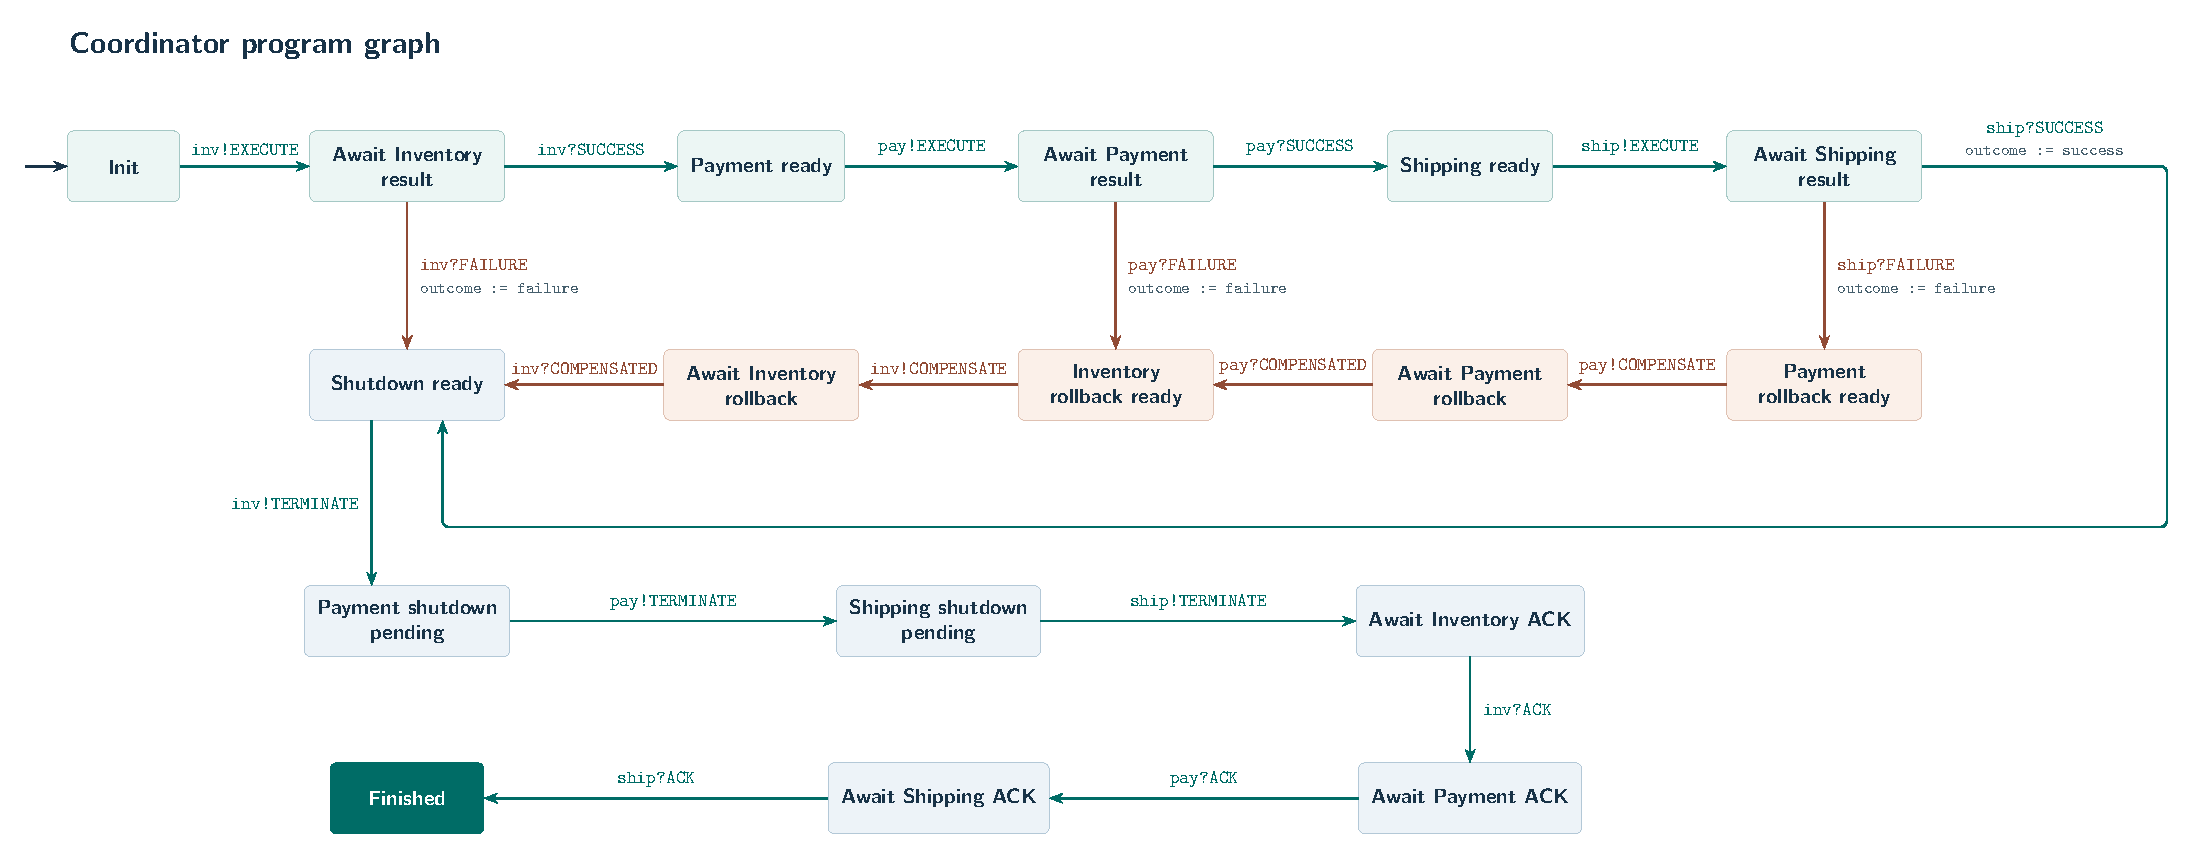
\includegraphics[page=1,width=\linewidth]{CA1-Program-Graphs.pdf}
  \caption{Transaction Coordinator program graph.}
  \label{fig:coordinator-graph}
\end{figure}
\end{landscape}

\servicegraph{2}{Inventory Service program graph.}{fig:inventory-graph}
\servicegraph{3}{Payment Service program graph.}{fig:payment-graph}
\servicegraph{4}{Shipping Service program graph.}{fig:shipping-graph}

\end{document}
